\documentclass[aspectratio=169]{beamer}

\mode<presentation>
{
  \usetheme{default}
  \usecolortheme{default}
  \usefonttheme{default}
  \setbeamertemplate{navigation symbols}{}
  \setbeamertemplate{caption}[numbered]
  \setbeamertemplate{footline}[frame number]  % or "page number"
  \setbeamercolor{frametitle}{fg=white}
  \setbeamercolor{footline}{fg=black}
} 

\usepackage[english]{babel}
\usepackage[utf8x]{inputenc}
\usepackage{tikz}
\usepackage{courier}
\usepackage{array}
\usepackage{bold-extra}
\usepackage{minted}
\usepackage[thicklines]{cancel}

\xdefinecolor{dianablue}{rgb}{0.18,0.24,0.31}
\xdefinecolor{darkblue}{rgb}{0.1,0.1,0.7}
\xdefinecolor{darkgreen}{rgb}{0,0.5,0}
\xdefinecolor{darkgrey}{rgb}{0.35,0.35,0.35}
\xdefinecolor{darkorange}{rgb}{0.8,0.5,0}
\xdefinecolor{darkred}{rgb}{0.7,0,0}
\definecolor{darkgreen}{rgb}{0,0.6,0}
\definecolor{mauve}{rgb}{0.58,0,0.82}

% 20 minutes
\title[2018-03-27-analysis-systems]{Spark-like and query-like analysis systems and tools \\ \vspace{0.25 cm}(what works, what doesn't work, and what's needed)}
\author{Jim Pivarski}
\institute{Princeton University -- DIANA-HEP}
\date{March 27, 2018}

\begin{document}

\logo{\pgfputat{\pgfxy(0.11, 7.4)}{\pgfbox[right,base]{\tikz{\filldraw[fill=dianablue, draw=none] (0 cm, 0 cm) rectangle (50 cm, 1 cm);}\mbox{\hspace{-8 cm}
\includegraphics[height=1 cm]{princeton-logo-long.png}
\includegraphics[height=1 cm]{diana-hep-logo-long.png}}}}}

\begin{frame}
  \titlepage
\end{frame}

\logo{\pgfputat{\pgfxy(0.11, 7.4)}{\pgfbox[right,base]{\tikz{\filldraw[fill=dianablue, draw=none] (0 cm, 0 cm) rectangle (50 cm, 1 cm);}\mbox{\hspace{-8 cm}
\includegraphics[height=1 cm]{princeton-logo.png}
\includegraphics[height=1 cm]{diana-hep-logo.png}}}}}

% Uncomment these lines for an automatically generated outline.
%\begin{frame}{Outline}
%  \tableofcontents
%\end{frame}

% START START START START START START START START START START START START START

\begin{frame}{``Analysis system'' as an optimization point}
\vspace{0.25 cm}
\begin{block}{Assumptions about access:}
\begin{itemize}\setlength{\itemsep}{0.35 cm}
\item Only need a small fraction of the event and particle attributes, like a few dozen.

\vspace{0.1 cm}
\textcolor{gray}{(A handful of trigger booleans, details on two or three particle types, maybe a veto on one or two more, but nowhere close to the thousands of attributes that exist.)}

\item Need to look at all events, if only to reject them on the basis of a few attributes.

\item Frequent, repeated process; code to run not known in advance; exploratory.
\end{itemize}
\end{block}

\begin{uncoverenv}<2->\begin{block}{Many analyses fit these conditions, but today's pipelines were designed for a different optimization point: reconstruction.}
\vspace{0.25 cm}
\uncover<3>{Consider this request: ``Please submit a GRID job to plot the muon kinematics. Then we'll think about what we want to look at next.'' Is that unreasonable?}
\end{block}
\end{uncoverenv}
\end{frame}

\begin{frame}{An example of what I have in mind: Google BigQuery}
\vspace{0.25 cm}
\begin{columns}
\column{1.1\linewidth}
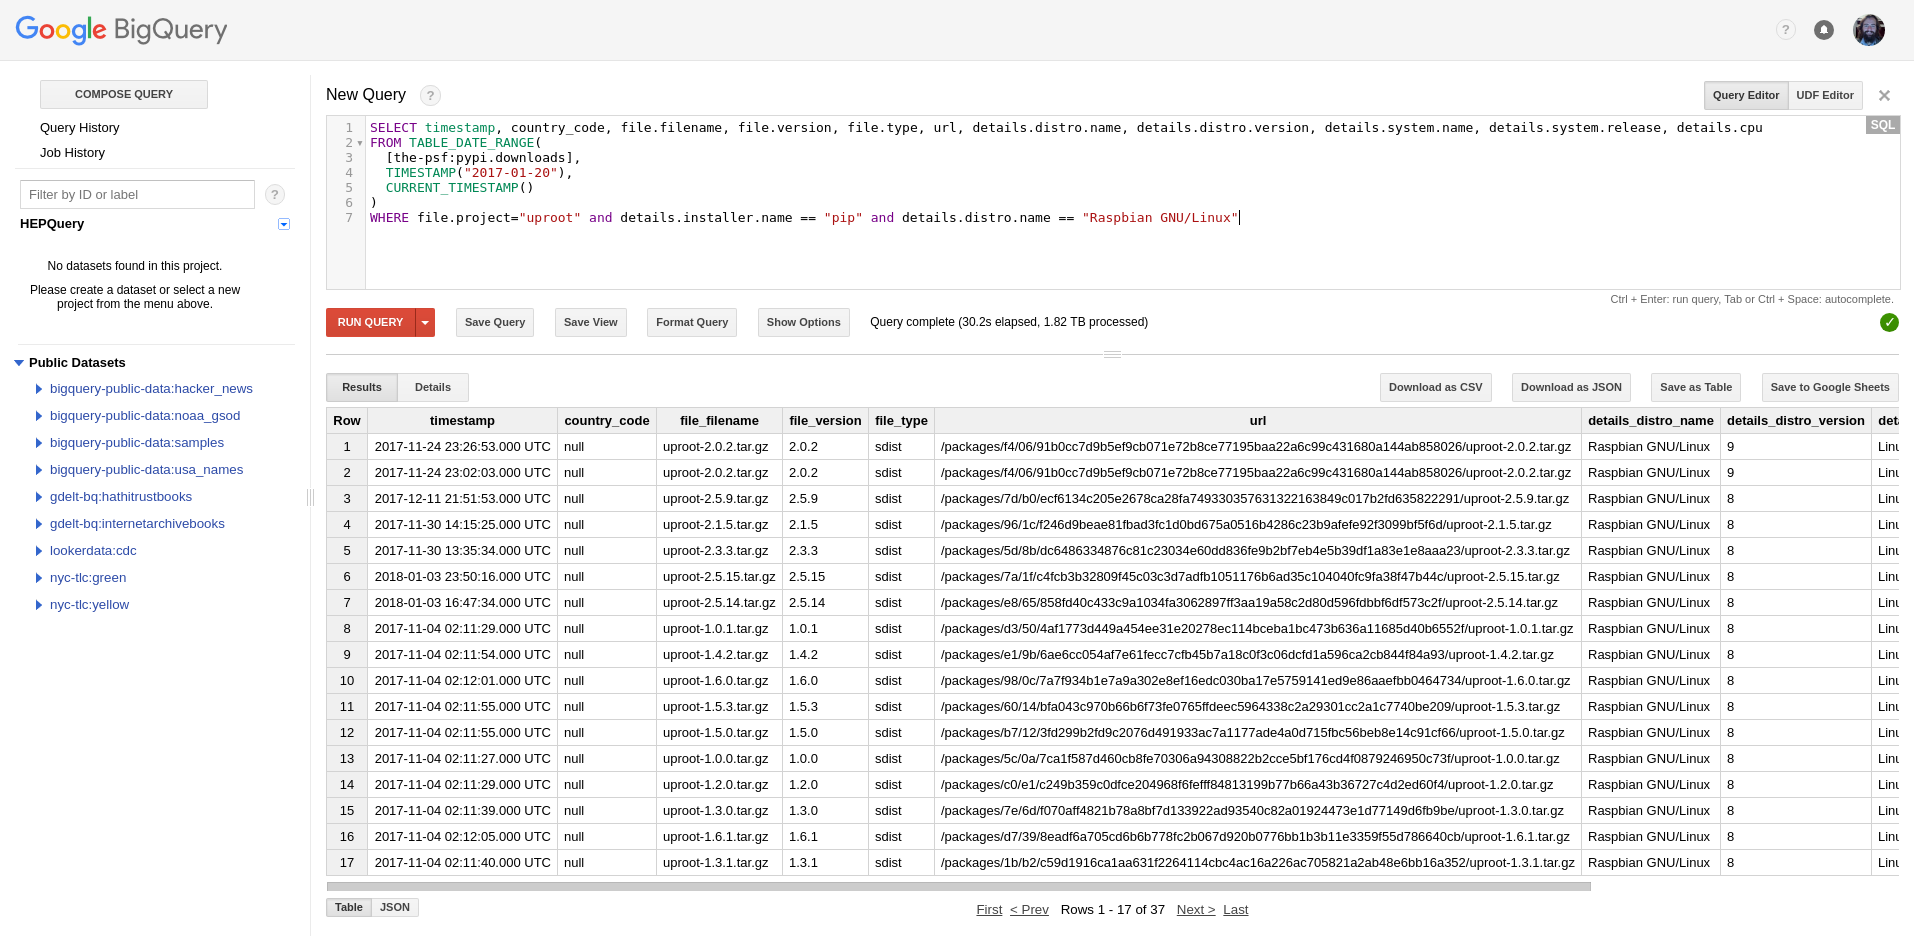
\includegraphics[width=\linewidth]{bigquery.png}
\end{columns}
\end{frame}

\begin{frame}{Basic block diagram}
\vspace{0.25 cm}
\begin{center}
\only<1-2>{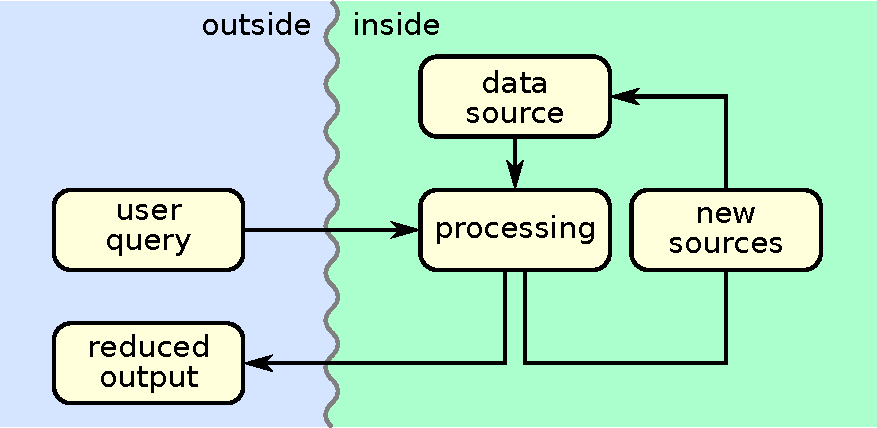
\includegraphics[width=0.7\linewidth]{basic-block-diagram.pdf}}
\only<3>{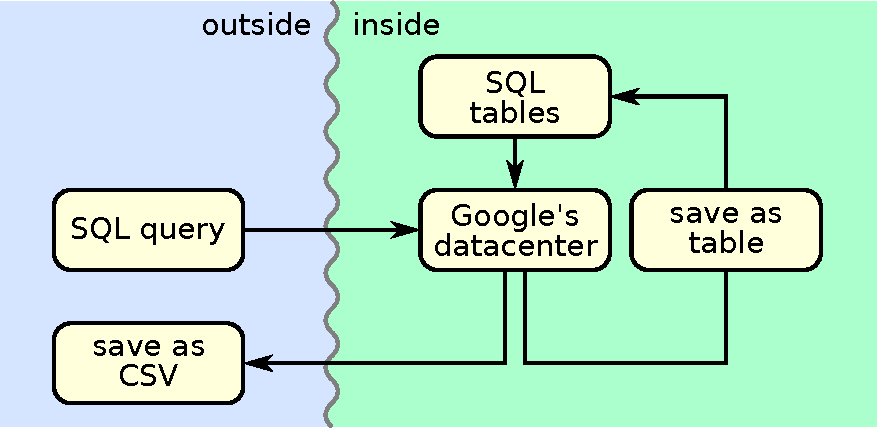
\includegraphics[width=0.7\linewidth]{google-block-diagram.pdf}}
\end{center}

\begin{uncoverenv}<2->
The ``new sources'' can be arbitrarily large and efficiently share overlapping data with the original sources because they live in the same system.

\vspace{0.25 cm}
The ``reduced output'' must be small enough to download quickly (e.g.\ histograms or highly skimmed tables). If not, the system ceases to be ``exploratory.''
\end{uncoverenv}
\end{frame}

\begin{frame}{So we can just use BigQuery, then?}
\vspace{0.25 cm}
\mbox{ } \hfill \textcolor{red}{\Huge No!!!} \hfill \mbox{ }

\vspace{0.1 cm}
\begin{itemize}\setlength{\itemsep}{0.2 cm}
\item<2-> \textcolor{darkblue}{Reason \#1: SQL.} Simple HEP problems translate into complex SQL and moderate-to-complex HEP problems would be unreasonably difficult to express.

\vspace{0.15 cm}
Non-SQL languages in this problem space, such as SparkSQL's column expressions or Apache Drill's internal query language, are just as restrictive in the ways that matter.

\item<3-> \textcolor{darkblue}{Reason \#2: Data model.} The BigQuery paper (``Dremel''), Parquet \& Drill (open source versions of the same), Apache Arrow, and SparkSQL all describe rich, nested data models sufficient to describe HEP events.

\vspace{0.15 cm}
However, {\it for every one of these,} you quickly encounter ``not implemented yet'' messages when you try to use them for HEP events.

\item<4-> \textcolor{darkblue}{Reason \#3: User interface.} The web form is fun, but we need queries embedded in an interactive, programmable environment with plotting and statistics libraries: ROOT or Python or both (probably both).
\end{itemize}
\end{frame}

\begin{frame}{HEP data are both simpler and more complex than others}
\vspace{0.35 cm}
\mbox{ } \hfill \textcolor{red}{\LARGE Simpler:} \hfill \mbox{ }

\vspace{0.25 cm}
\begin{columns}
\column{0.5\linewidth}

HEP functions never have to cross events.

\vspace{0.25 cm}
\mbox{ } \hfill 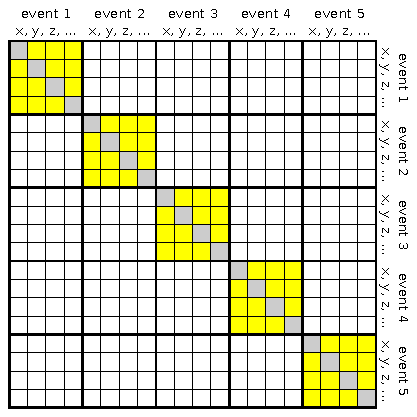
\includegraphics[width=0.8\linewidth]{event-variable-correlation-hep.pdf} \hfill \mbox{ }

\column{0.5\linewidth}

\mbox{\hspace{-0.5 cm}Common elsewhere: e.g.\ market basket analysis.\hspace{-0.5 cm}}

\vspace{0.25 cm}
\mbox{ } \hfill 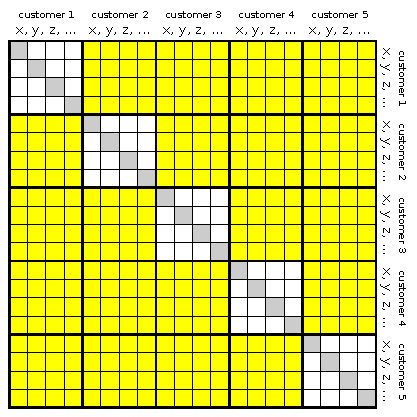
\includegraphics[width=0.8\linewidth]{event-variable-correlation-marketbasket-2.pdf} \hfill \mbox{ }

\end{columns}
\end{frame}

\begin{frame}{HEP data are both simpler and more complex than others}
\vspace{0.35 cm}
\mbox{ } \hfill \textcolor{red}{\LARGE More complex:} \hfill \mbox{ }

\vspace{-0.25 cm}
\begin{columns}[t]
\column{0.5\linewidth}

HEP data are variable-length, nested data structures, and we typically need to loop over combinations of particles.

\vspace{0.25 cm}
\mbox{ } \hfill 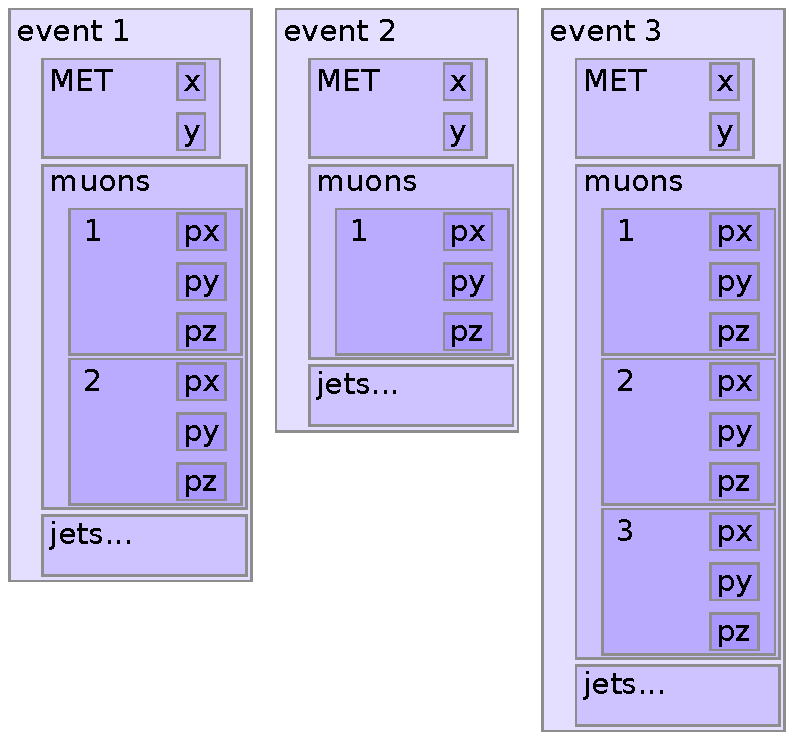
\includegraphics[width=0.8\linewidth]{event-structure.pdf} \hfill \hfill \mbox{ }

\column{0.5\linewidth}

In most fields, data are not considered ready for analysis until they're in a tabular form. (Earlier steps are called ``tidying.'')

\vspace{0.25 cm}
\mbox{ } \hfill 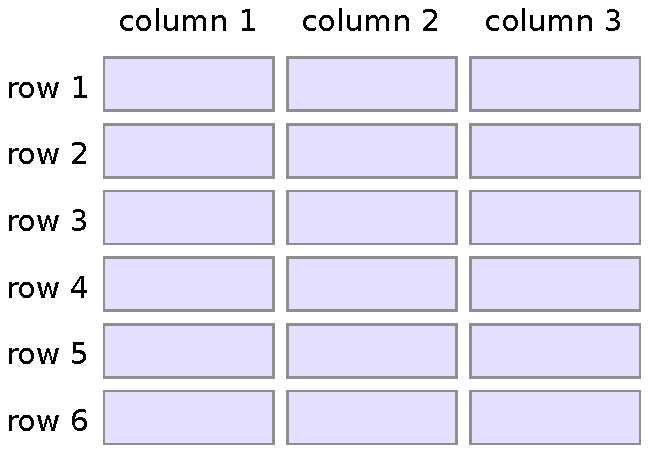
\includegraphics[width=0.8\linewidth]{table-structure.pdf} \hfill \hfill \mbox{ }

\end{columns}
\end{frame}



\end{document}
